\documentclass[a4paper,10pt]{article}
\usepackage[utf8]{inputenc}
\usepackage{amsmath}
\usepackage{amssymb}
\usepackage{fullpage}
\usepackage{subfigure}
\usepackage{graphicx}
\usepackage{array}
\usepackage{floatrow}
\usepackage{color, colortbl}
\usepackage{placeins} % for FloatBarrier
\usepackage{algorithm}
\usepackage{algorithmic}
\definecolor{Gray}{gray}{0.9}

%opening
\def\sscale{0.7}
\def\figh{2in}
\def\bfigh{3in}
\def\1{^{\prime}}
\def\T{\mathcal{T}}
%\def\tT{\widetilde\T}
\def\tT{\T\1}
\def\Y{\mathcal{Y}}
\def\C{\mathcal{C}}
\def\U{\mathcal{U}}
\def\R{\mathcal{R}}
\def\S{\mathcal{S}}
\def\NN{\mathbb{N}}
\def\nop{\text{nop}}
\def\ang#1{\left\langle#1\right\rangle}
\def\qtx#1{\quad\text{#1}\quad}
\def\andn{\setminus}
\def\inv{^{-1}}

\def\seq{\operatorname{Sequences}}
\def\Rep{\operatorname{Rep}}
\def\Comp{\operatorname{Comp}}
\def\Adj{\operatorname{Adj}}

\newtheorem{example}{Example}
\newtheorem{definition}{Definition}
\newtheorem{notation}{Notation}
\newtheorem{lemma}{Lemma}

\renewcommand{\algorithmicrequire}{\textbf{Input:}}
\renewcommand{\algorithmicensure}{\textbf{Output:}}

\begin{document}
\section{Formalization}
Let $\Y$ be a set of observations and $\U$ a set of control actions.
The original formalization defines a decision table as a map $\T:\C\to\U$, where $\C=\bigcup_{i=1}^n\Y^i$ for some $n\in\NN$.  
This definition is often stronger than necessary, as there may be contexts $c$
in which certain observations $y\in\Y$ are never encountered.  In such a context, any assignment $\T(c)\in\U$,
produces the same policy, although the choice of $\T(c)$ can affect a policy's reducibility.
\begin{example}[Equivalent Decision Tables] \label{ex:complete}
Suppose $\Y=\{1,2\}$, $\U=\{A,B\}$, $\C=\bigcup_{i=1}^2\Y^i$ and 
$$\T(c) = \begin{cases}
A & c \in \{(1), (1,2)\}\\
B & c \in \{(2), (2,1)\}\\
\tT(c) & \text{otherwise.}
\end{cases},$$
is an optimal policy, for arbitrary $\tT:\C\to\U$. However, depending on the choice of $\tT$ (highlighted in the tables below),
the completed policy can have differently-sized minimal representations:

\begin{figure}[h]
\begin{floatrow}
\subfigure[Decision Table]{
\ffigbox[\FBwidth]{
\begin{tabular}{ll}
\rlap{$\T:\C\to\U$}\\
\hline
$(1)$&$\mapsto A$\\
$(2)$&$\mapsto B$\\
\rowcolor{Gray}
$(1,1)$&$\mapsto A$\\
$(1,2)$&$\mapsto A$\\
$(2,1)$&$\mapsto B$\\
\rowcolor{Gray}
$(2,2)$&$\mapsto B$
\end{tabular}
}{}}\quad
\subfigure[Decision Tree]{
\ffigbox[\FBwidth]{
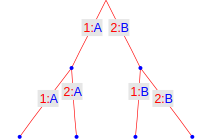
\includegraphics[scale=\sscale]{media/overcomplete_decision}
}{}}\quad\quad
\subfigure[Minimal Policy]{
\ffigbox[\FBwidth]{
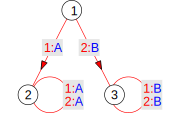
\includegraphics[scale=\sscale]{media/overcomplete-2}
}{}}
\end{floatrow}
\bigskip

\begin{floatrow}
\subfigure[Decision Table]{
\ffigbox[\FBwidth]{
\begin{tabular}{ll}
\rlap{$\T:\C\to\U$}\\
\hline
$(1)$&$\mapsto A$\\
$(2)$&$\mapsto B$\\
\rowcolor{Gray}
$(1,1)$&$\mapsto B$\\
$(1,2)$&$\mapsto A$\\
$(2,1)$&$\mapsto B$\\
\rowcolor{Gray}
$(2,2)$&$\mapsto A$
\end{tabular}
}{}}\quad
\subfigure[Decision Tree]{
\ffigbox[\FBwidth]{
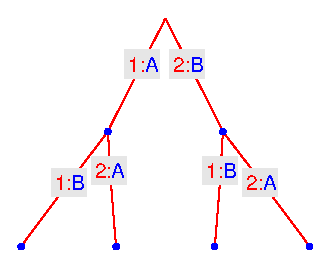
\includegraphics[scale=\sscale]{media/complete_decision}
}{}}\quad\quad
\subfigure[Minimal Policy]{
\hspace{.2cm}
\ffigbox[\FBwidth]{
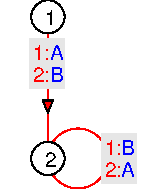
\includegraphics[scale=\sscale]{media/complete-2}
\setcounter{figure}{\value{example}}
\label{fig:best_completion}
}{}}
\end{floatrow}
\end{figure}
\end{example}
Instead, we propose an ``incompletely-determined'' formalization:
\begin{definition}[Policies]
Given a set $\Y$ of observations, recursively construct
\begin{equation}
\C_0 = \{\emptyset\}\qtx{and}\C_{i+1} = \{(c,y_{i+1})\,:\,c\in\C_i,\, y_{i+1}\in\Y_c\},
\end{equation}
where $\Y_c\subseteq\Y$ are the observations that may be seen in context $c$.  
Let $\C = \bigcup_{i=0}^{\infty}\C_i$.
A \textbf{policy} $P$ is then a tuple $\ang{\C, \U, \T, \Y}$, 
where $\U$ is some decision set and $\T:\C\andn\{\emptyset\}\to\U$.
\end{definition}
\begin{definition}[Completely-Determined Policies]
If $\Y=\bigcup_\C\Y_c$ and $\C=\Y^{\leq n}$ for some $n\in\NN$, then $P=\ang{\C,\U,\T,\Y}$ is \textbf{completely determined}.
A \textbf{completion} of $P$ is a policy $P\1=\ang{\C\1, \U\1, \T\1, \Y}$ such that
\begin{equation}
\Y\subseteq\Y\1,\quad \C\1=\bigcup_{i=0}^{\infty}(\Y\1)^i,\quad \U\subseteq\U\1, \qtx{and} \T\1|_{\C} = \T.
\end{equation}
Let $\Comp(P)$ be the set of completions of the policy $P$.
\end{definition}
\begin{definition}[FSM Representations]
An \textbf{FSM representation} (or just \textbf{representation})
is a tuple $\ang{\C,\R,\U,\S,\T,\Y}$ (abbreviated to $\ang{\R,\S}$ when $P=\ang{\C,\U,\T,\Y}$ is given), 
with ``states'' $\S\subseteq\NN$ and state assignments $\R:\C\to\S$, such that 
\begin{equation}
\R(c)=\R(c\1)\qtx{and}y\in\Y_c\cap\Y_{c\1}\implies\T(c,y)=\T(c\1,y).
\end{equation} 
Let $\Rep(P)$ be the set of representations of the policy $P$.  
\end{definition}
\begin{definition}[Minimal Representations]
The \textbf{size} of an FSM representation is the cardinality of its state set.  
A representation $\ang{\R,\S}$ of $P$ is \textbf{minimal} if 
$|\S|=\min\{|\S\1|\,:\,\ang{\R\1,\S\1}\in\Rep(P)\}$.
A representation $\ang{\R\1,\S\1}$ is a \textbf{reduction} of the representation $\ang{\R,\S}$ if there is a surjection $\phi:\S\to\S\1$
such that $\R\1 = \phi(\R)$.
\end{definition}
\begin{example}
\label{ex:canon}
If $\C = \{c_1, c_2, \ldots\}$, then 
%for any policy $P=\ang{\C,\U,\T,\Y}$,
we have a canonical representation $\ang{\R,\S}$, where
\begin{equation}
\S=\{1,\ldots,|\C|\}\qtx{and}\R:c_k\mapsto k.
\end{equation} 
\end{example}
It can be shown that the size of a minimal representation of a policy $P$ is equal to the minimum
size of the minimal representations of its completions, i.e.
\begin{align}
\min\{|\S\1|\,:\,\ang{\R\1,\S\1}\in\Rep(P)\} = \min\{|\S\1|\,:\,\ang{\R\1,\S\1}\in\Rep(P\1),\,P\1\in\Comp(P)\}
\end{align}
Incompletely-determined policies allow more freedom in representation reduction, as shown in the next example.

\begin{example}[Incompletely-Determined Policies]
Let $\C=\{\emptyset, (1), (2), (1,2), (2,1)\}$, $\U=\{A,B\}$, and
\begin{equation*}
\T(c,y) = \begin{cases}
A & c\in\{(1), (1,2)\}\\
B & c\in\{(2), (2,1)\}
\end{cases}.
\end{equation*}
Observe that the minimal policy is the same as that of the completely-determined policy in Example \ref{fig:best_completion}.
\setcounter{subfigure}{0}
\begin{figure}[h]
\begin{floatrow}
\subfigure[Decision Table]{
\ffigbox[\FBwidth]{
\begin{tabular}{ll}
\multicolumn{2}{c}{$\T:\C\andn\{\emptyset\}\to\U$}\\
\hline
$(1)$&$\mapsto A$\\
$(2)$&$\mapsto B$\\
$(1,2)$&$\mapsto A$\\
$(2,1)$&$\mapsto B$\\
\end{tabular}
}{}}\qquad\quad
\subfigure[Decision Tree]{
\ffigbox[\FBwidth]{
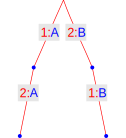
\includegraphics[scale=\sscale]{media/simple_decision}
}{}}\qquad\qquad
\subfigure[Representation]{
\ffigbox[\FBwidth]{
\begin{tabular}{ll}
\rlap{$\R:\C\to\S$}\\
\hline
$\emptyset$&$\mapsto 1$\\
$(1)$&$\mapsto 2$\\
$(2)$&$\mapsto 2$\\
$(1,2)$&$\mapsto 2$\\
$(2,1)$&$\mapsto 2$\\
\end{tabular}
}{}}\qquad\quad
\subfigure[Minimal Policy]{
\ffigbox[\FBwidth]{
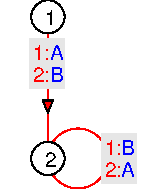
\includegraphics[scale=\sscale]{media/complete-2}
}{}}
\end{floatrow}
\setcounter{figure}{\value{example}}
\label{fig:incomplete}
\end{figure}
\end{example}
\section{Algorithm}

To find a minimum representation of a given policy,
we first compute a graph of reducibility relations, 
then compute a minimal clique-covering.
\setcounter{subfigure}{0}
\begin{figure}[ht]
\centering
\begin{floatrow}
\subfigure[Canonical Representation]{
\ffigbox[\FBwidth]{
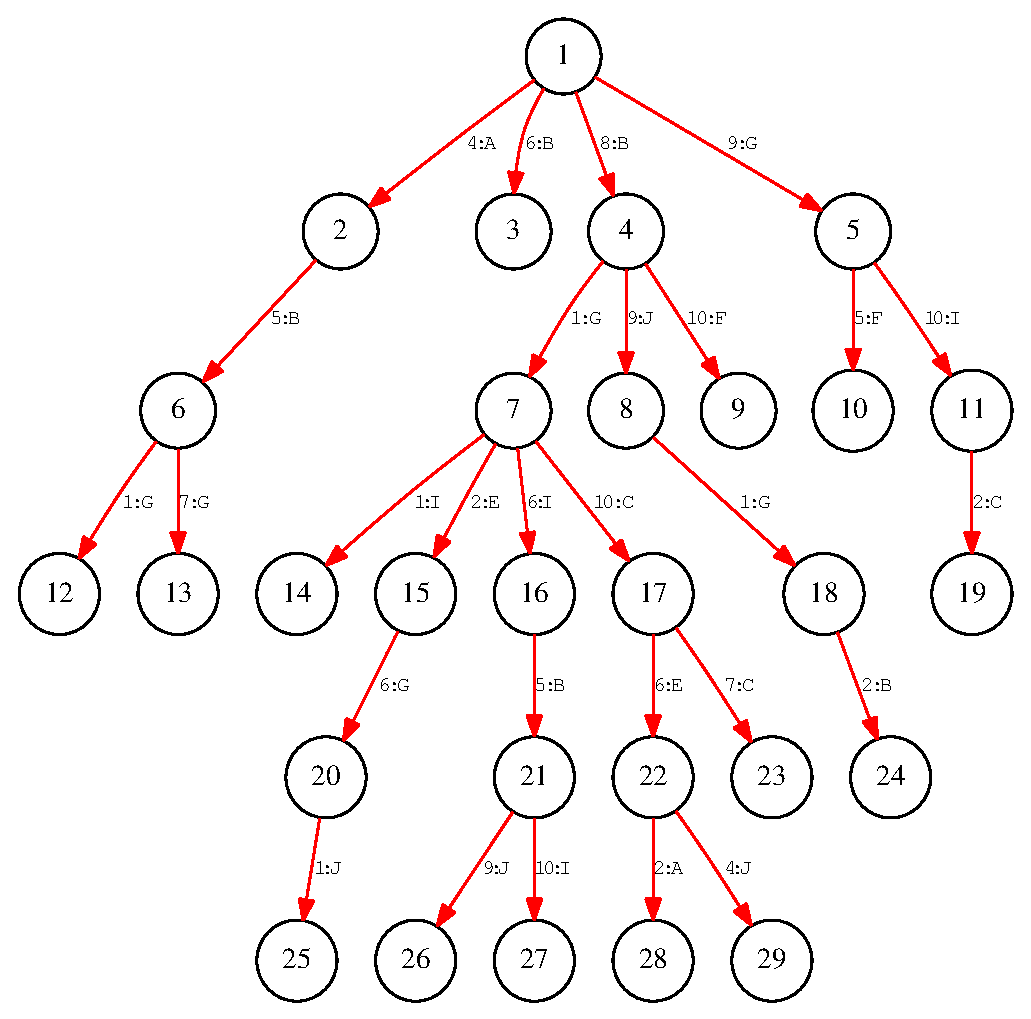
\includegraphics[height=\bfigh]{media/random_alg-1}
}{}}
\subfigure[Compatibility Matrix]{\label{fig:cgam}
\ffigbox[\FBwidth]{
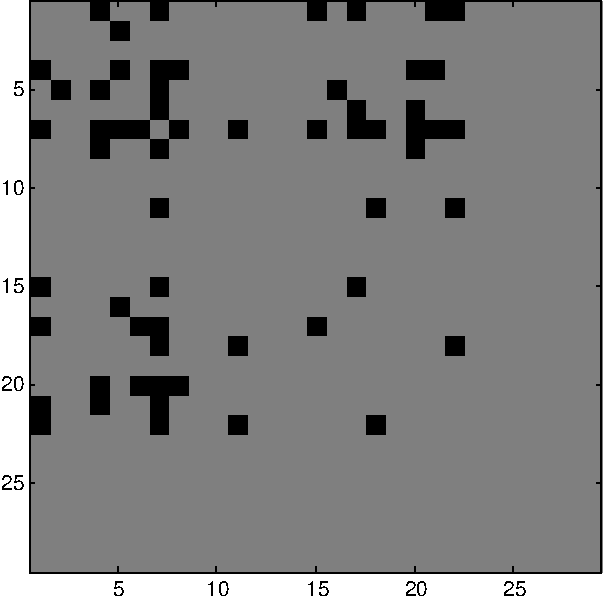
\includegraphics[height=\bfigh]{media/random_adj}
}{}}
\end{floatrow}
\end{figure}
\begin{figure}[ht]
\begin{floatrow}
\subfigure[Greedy Clique Covering of \ref{fig:cgam}]{
\ffigbox[\FBwidth]{
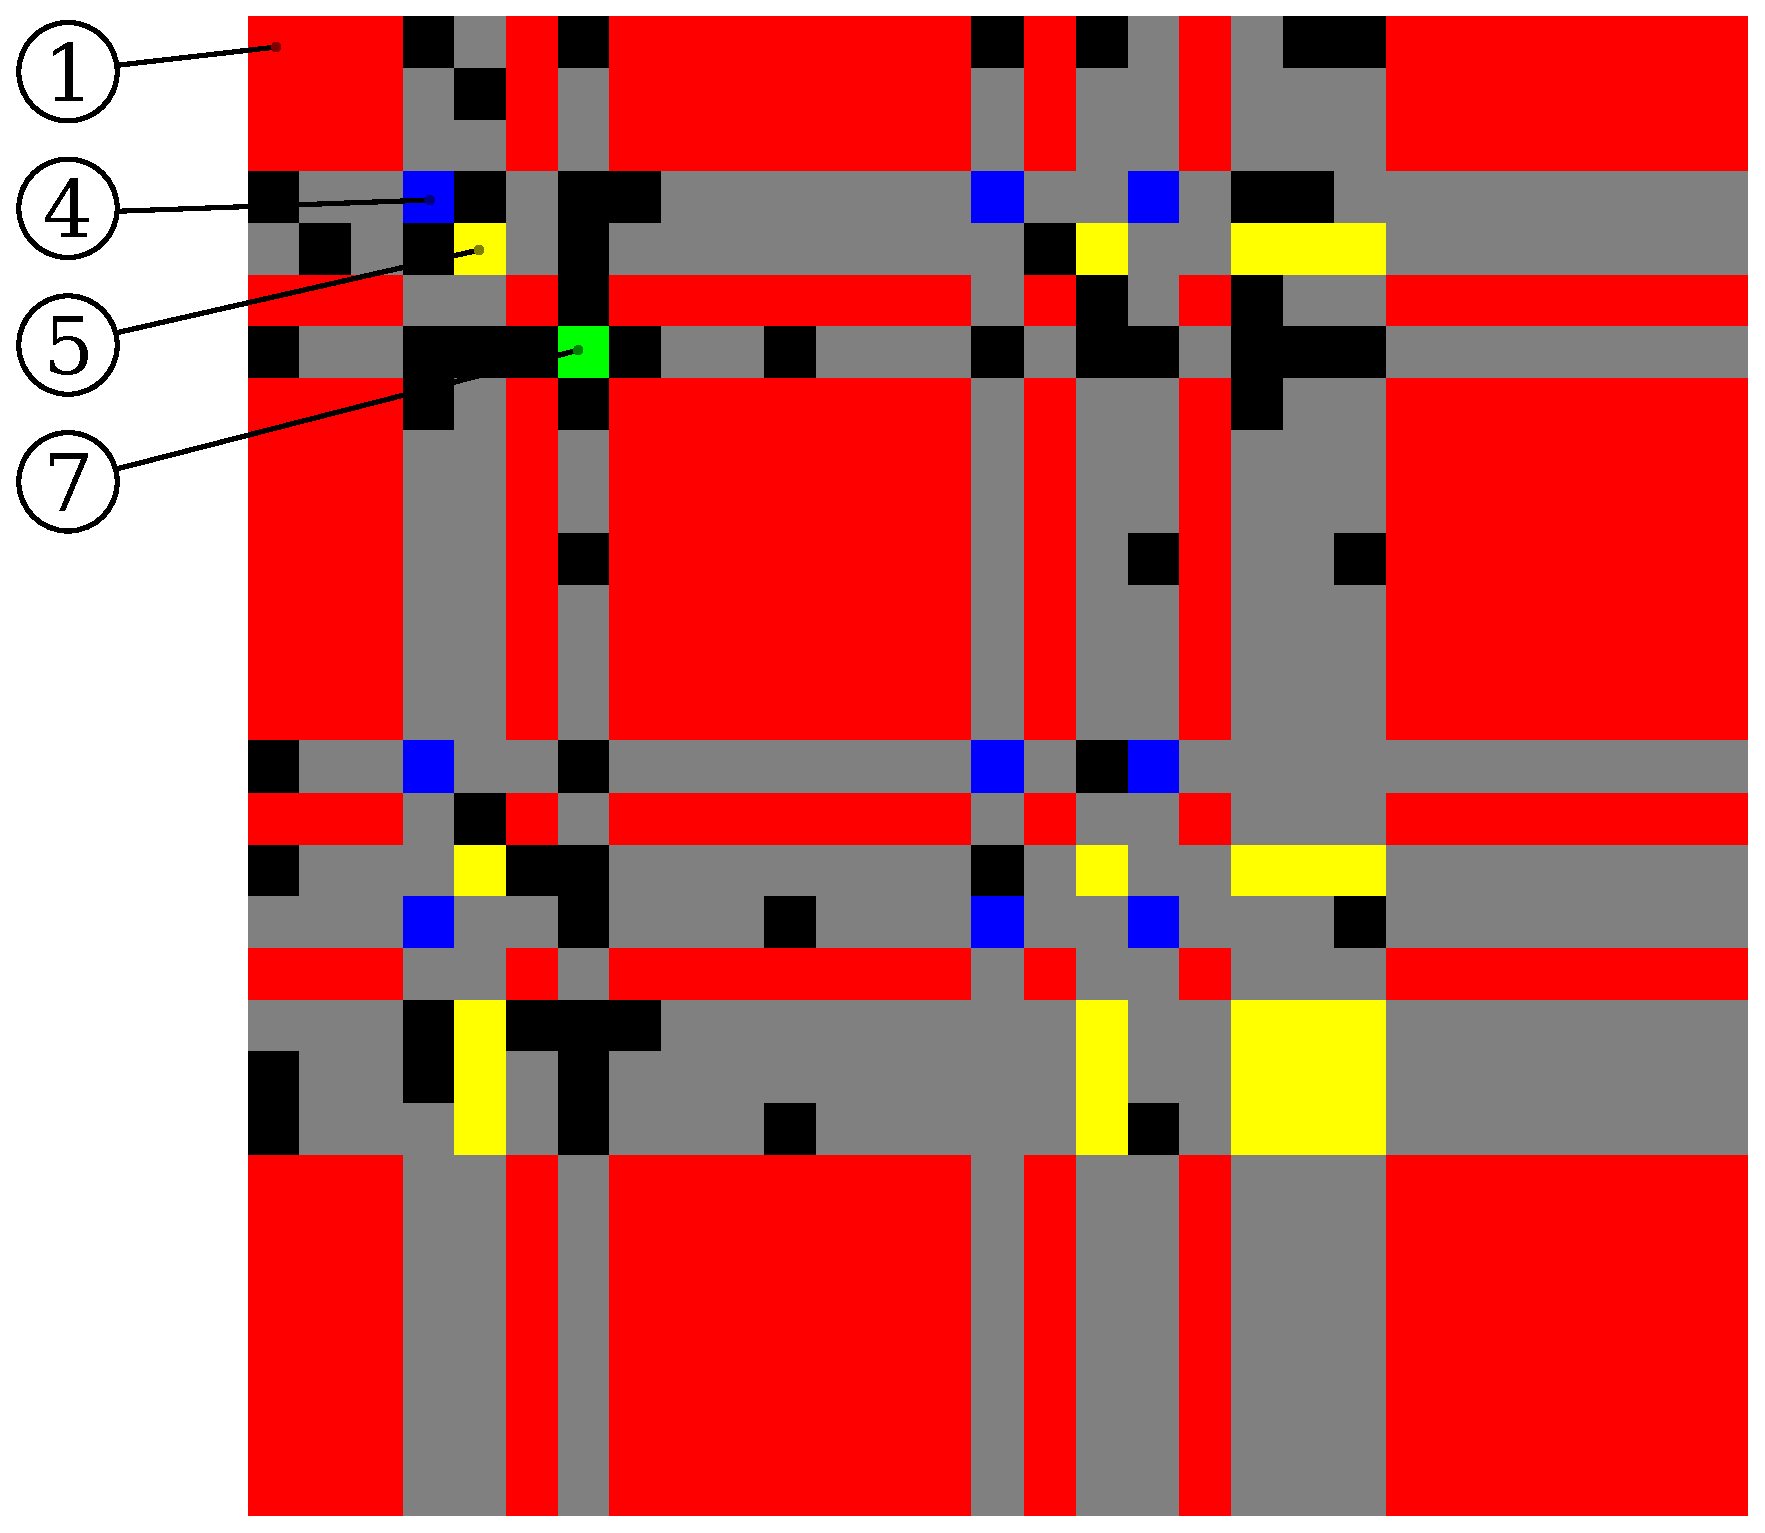
\includegraphics[height=\bfigh]{media/random_cliques}
}{}}\qquad
\subfigure[Reduced Representation]{
\ffigbox[\FBwidth]{
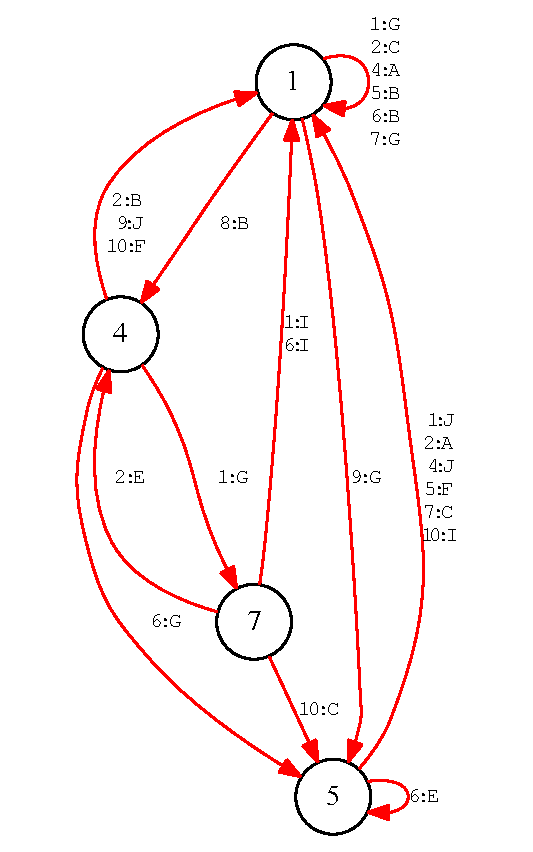
\includegraphics[height=\bfigh]{media/random_alg-2}
}{}}
\end{floatrow}
\end{figure}
For practical computation of reducibility, we'll start with the weaker condition of compatibility.

\subsection{Reducibility Relations}

\begin{definition}[Reducibility]
For a given policy $P=\ang{\C,\U,\T,\Y}$, two contexts $c_1, c_2\in\C$ are \textbf{reducible} (write $c_1\sim c_2$) if there exists a representation 
$\ang{\R,\S}$ of $P$ such that $\R(c_1)=\R(c_2)$.  Likewise, for a given representation $R=\ang{\R,\S}$, two states 
$s_1,s_2\in\S$ are \textbf{reducible} if there exists a reduction $(\phi, \ang{\R\1,\S\1})$ of $R$ such that
$\phi(s_1)=\phi(s_2)$.
\end{definition}
Observe that for any representation $\ang{\C,\R,\U,\S,\T,\Y}$,
the contexts $c_1, c_2\in\C$ are reducible if and only if the states $\R(c_1)$ and $\R(c_2)$ are reducible.
Observe also that for incompletely-determined policies, reducibility is a symmetric but not-necessarily-transitive relation
\begin{example}[Non-Transitive Reducibility]
Suppose $\Y=\{1,2,3\}$, $\C=\{\emptyset, (1), (2), (1,3), (2,3)\}$, \mbox{$\U=\{A,B\}$}, and 
\begin{equation}
\T(c) = \begin{cases}
A&c\in\{(1), (1,3)\}\\
B&c\in\{(2), (2,3)\}
\end{cases}.
\end{equation} 
Observe that, under this policy, $\emptyset\sim(1)$ and $\emptyset\sim(2)$, but $(1)\not\sim(2)$, 
since $\T(1,3)\neq\T(2,3)$.
\end{example}
However, it can be shown that, under a completely-determined policy, reducibility induces an equivalence relation.  
In either case, we compute reducibility using the following criterion:
\begin{lemma}
Two contexts $c_1,c_2\in\C$ are reducible iff 
\begin{equation}
\T(c_1,s)=\T(c_2,s)\qtx{for all}s\in\Y^*\qtx{such that}(c_1,s),(c_2,s)\in\C
\end{equation} 
\end{lemma}

This informs the following algorithm
\begin{algorithm}                      % enter the algorithm environment
\caption{Compute Reducibility Relations}          % give the algorithm a caption
\label{alg1}                           % and a label for \ref{} commands later in the document
\begin{algorithmic}                    % enter the algorithmic environment
  \REQUIRE A representation $\ang{\C,\R,\U,\S,\T,\Y}$
  \ENSURE A reducibility matrix $A:\S\times\S\to\{\TRUE,\FALSE\}$.
  \bigskip
  
  \STATE $A(s_1, s_2)\Leftarrow \TRUE$\quad for all $s_1,s_2\in\S$.
  \REPEAT
    \STATE $isChanged \Leftarrow \FALSE$
    \FOR{$s_1<s_2\in \S$}
	  
	  \IF{$A(s_1,s_2)=\TRUE$}
		\FOR{$c_1\in\R\inv(s_1),\,c_2\in\R\inv(s_2)$}
		  \FOR{$y\in\Y_{c_1}\cap\Y_{c_2}$}
			\IF{$\T(c_1,y)\neq\T(c_2,y)\;\;\text{or}\;\;^{\sim}A(\R(c_1,y),\R(c_2,y))$}
			  \STATE $A(s_1,s_2)\Leftarrow\FALSE$.
			  \STATE $isChanged\Leftarrow\TRUE$.
			\ENDIF
		  \ENDFOR
		\ENDFOR
	  \ENDIF
    \ENDFOR
  \UNTIL{$^{\sim}isChanged$} 
\end{algorithmic}
\end{algorithm}

Now, although reducibility is not an equivalence relation, 
any reduction $\phi:\S\to\S\1$ induces an equivalence relation,
partitioning $\S$ into cliques of mutually-reducible states, i.e.
\begin{equation}
\S = \bigsqcup_{s\1\in\S\1}\phi\inv(s\1),\qtx{where}\phi(s_1)=\phi(s_2)\implies A(s_1,s_2)
\end{equation}
Thus, a minimal reduction
induces a minimal clique partition of the
reducible states of a representation.
\subsection{Assembling Cliques}
\begin{notation}[Arrow notation]
For a policy $P=\ang{\C,\U,\T,\Y}$, 
write $c\to c\1$ if $c=(c_1,\ldots,c_i)\in\C_i\subseteq\C$ and 
$c\1=(c_1,\ldots,c_i,y)\in\C_{i+1}\subseteq\C$, for some $i$.  For a representation $\ang{\R,\S}$ of $P$,
write $s_1\to s_2$ if there are $c_1\in f\inv(s_1)$ and $c_2\in f\inv(s_2)$ such that $c_1\to c_2$.
\end{notation}
We propose the following, greedy, approximate algorithm
\begin{algorithm}                      % enter the algorithm environment
\caption{Compute Clique Covering}          % give the algorithm a caption
\label{alg2}                           % and a label for \ref{} commands later in the document
\begin{algorithmic}                    % enter the algorithmic environment]
  \REQUIRE A representation $\ang{\C,\R,\U,\S,\T,\Y}$ with $s_1<s_2$ only if $s_2\not\to s_1$.
  \REQUIRE A reducibility matrix $A:\S\times\S\to\{\TRUE,\FALSE\}$ as computed by Algorithm \ref{alg1}.
  \ENSURE A partition function $\phi:\S\to\S\1$ with $\phi(s_1)=\phi(s_2)$ only if $A(s_1,s_2)$.
  \bigskip
  
  \STATE $\S\1\Leftarrow\S$
  \STATE $\phi\Leftarrow id_{\S}$
  \STATE $unused\Leftarrow\S$
  \WHILE{$|unused|>0$}
	\STATE $s_1\Leftarrow\min(unused)$
	\STATE $unused\Leftarrow unused\andn\{s_1\}$
	\FOR{$s_2\in unused$}
	  \IF{$A(s_1,s_2)$}
		\STATE $\phi(s_2)\Leftarrow s_1$
		\STATE $unused\Leftarrow unused\andn\{s_2\}$
	  \ENDIF
	\ENDFOR
  \ENDWHILE
\end{algorithmic}
\end{algorithm}
Although we have no proof that this algorithm produces minimal representations
of a given policy, it is not inconceivable that this or another greedy policy could work.
In general, the Minimal Clique Covering problem is NP-Complete, 
but the tree structure of the decision policy is an a constraint that may simplify the problem.
\FloatBarrier

\section{Code}
The main MATLAB routine is in \texttt{decision\_script.m}.   
By default it generates a random decision tree, 
whose branching is governed by a Poisson distribution.

\subsection{Console Output}
\begin{verbatim}
Initial FSM:
---------------------------------------------------
01:  08-->(05, 02),  
02:  02-->(05, 03),  06-->(03, 04),  10-->(01, 05),  
03:  07-->(04, 06),  08-->(07, 07),  
04:  
05:  05-->(10, 08),  07-->(06, 09),  
06:  04-->(09, 10),  05-->(05, 11),  07-->(09, 12),  
07:  
08:  09-->(07, 13),  
09:  03-->(08, 14),  
10:  
11:  
12:  04-->(01, 15),  06-->(06, 16),  
13:  01-->(03, 17),  
14:  07-->(01, 18),  
15:  
16:  
17:  
18:  

Final clique covering: {1, 2, 4, 5, 7, 8, 9, 10, 11, 13, 15, 16, 17, 18}  {3, 12}  {6}  {14}  
\end{verbatim}

\subsection{Visualizations}

\setcounter{subfigure}{0}
\begin{figure}[h]
\centering
\subfigure[Original Policy]{
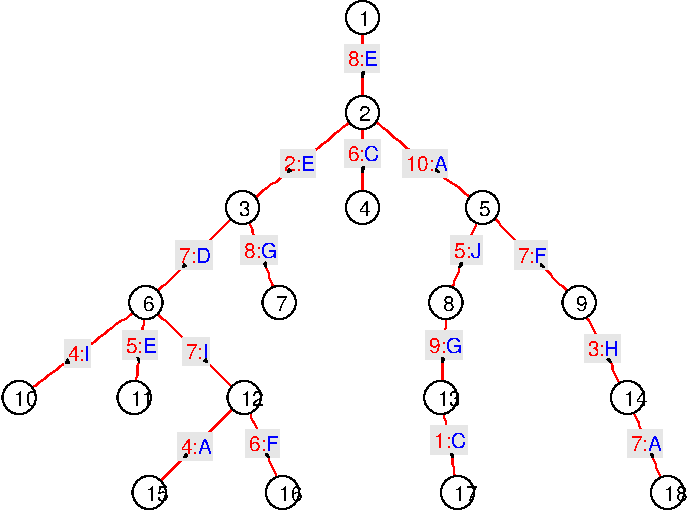
\includegraphics[height=\figh]{media/random_orig_mat}}\qquad\quad
\subfigure[Reduced Policy]{
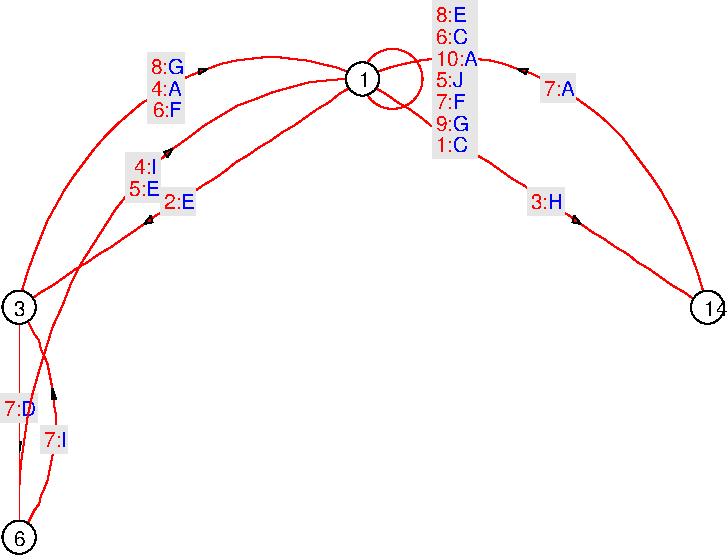
\includegraphics[height=\figh]{media/random_redu_mat}}
\caption{MATLAB Visualizations}
\end{figure}

An optional section of this script uses Graphviz to 
produce high-quality FSM visualizations.

\FloatBarrier
\begin{figure}[ht]
\centering
\subfigure[Original Policy]{
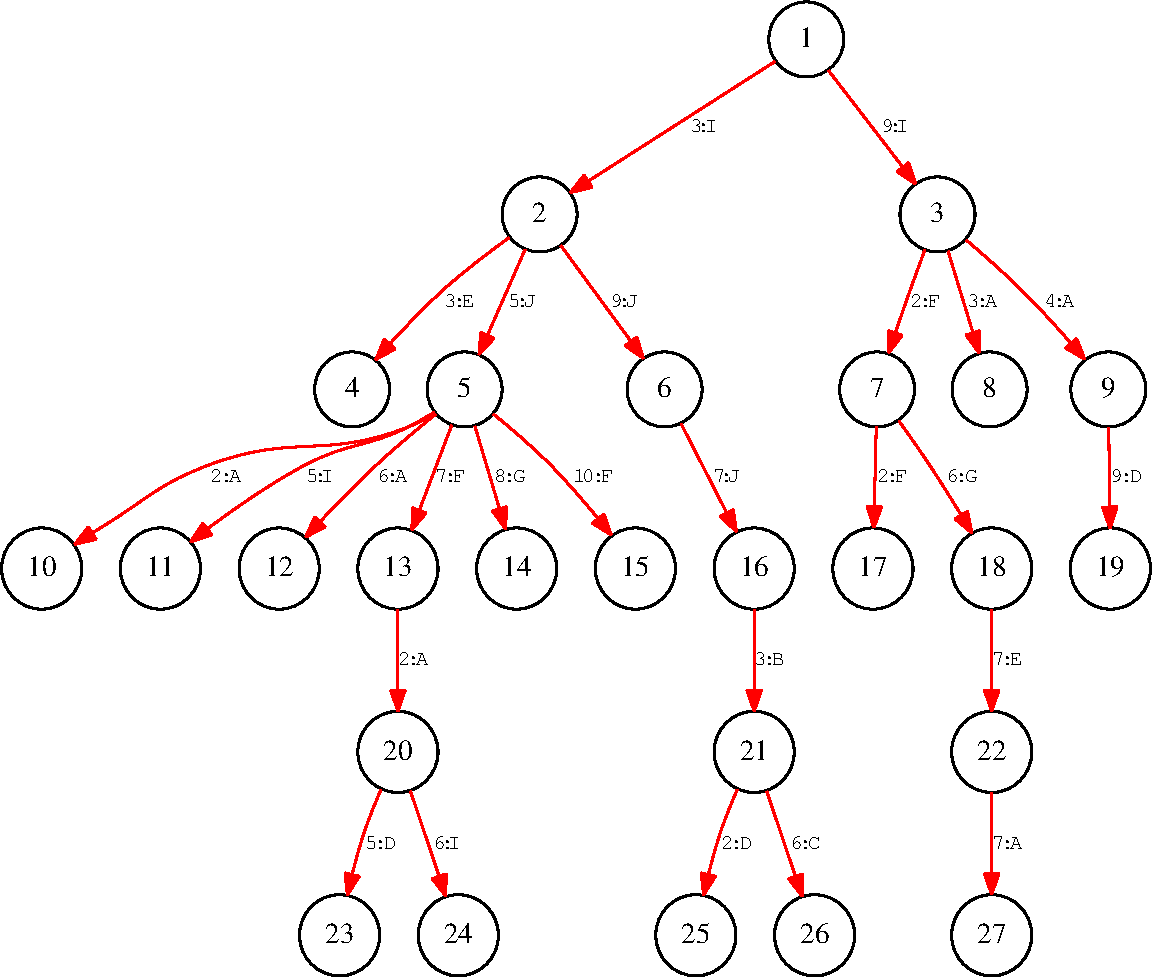
\includegraphics[height=\bfigh]{media/random_orig_gv}}\qquad\qquad
\subfigure[Reduced Policy]{
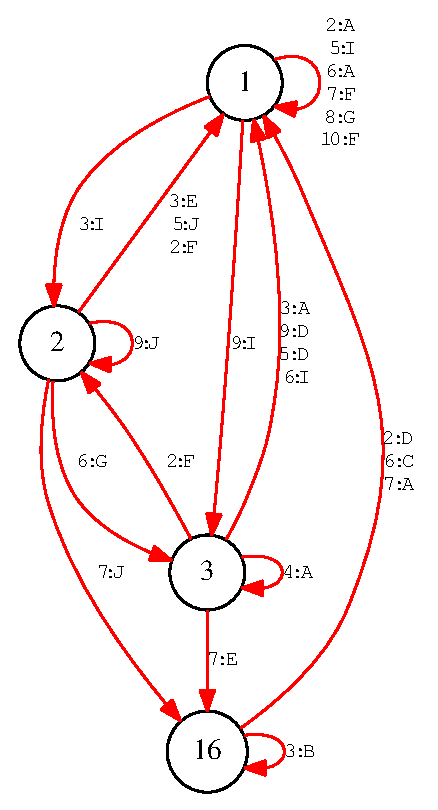
\includegraphics[height=\bfigh]{media/random_redu_gv}}
\caption{Graphviz Visualizations}
\end{figure}
\FloatBarrier
\noindent This makes a system call to the script \texttt{drawgraph.sh}, which runs in the bash shell,
and uses a few non-standard graphics utilities.  In Ubuntu, these dependencies should be 
resolved by the command
\begin{verbatim}
$ sudo apt-get install ghostscript texlive-extra-utils graphviz evince
\end{verbatim}


\end{document}
